\documentclass[../rapport.tex]{subfiles}
\graphicspath{{\subfix{ressources/photos_diagrammes/extensionChristian/}}}

\begin{document}
		\subsubsection{Vue d'ensemble}
		L'extension 6 Paiement et gestion des fraude a pour but de permettre a un client de générer des QRcode , de scanner des QRcode ( évènement simulé en pratique),\\
        effectuer des payments avec et sans contact(évènement simulé en pratique) et d'avoir un système de détetction de fraud permettant de restraindre ou dans certains cas de bloquer des transactions suspecte.\\
        Pour l'insitution cette extension implement un système de limites de transactions portant sur les payments avec et sans contact.\\
        Le plus gros des ajouts sont éffectué pour l'application 1 et donc les diagramme se basent fortement sur celle-ci.\\
        L'application 2 se vois n'ayant que la définitions de limites de payments, elle est quasiment identique a celle de base.\\
        Les ajouts éffectué au diagrammes des 2 applications sont démarqué par une couleur rose.\\

		\subsubsection{Application 1}

		\subsubsection{Diagramme des cas d'utilisation}
				\begin{figure}[h]
						\centering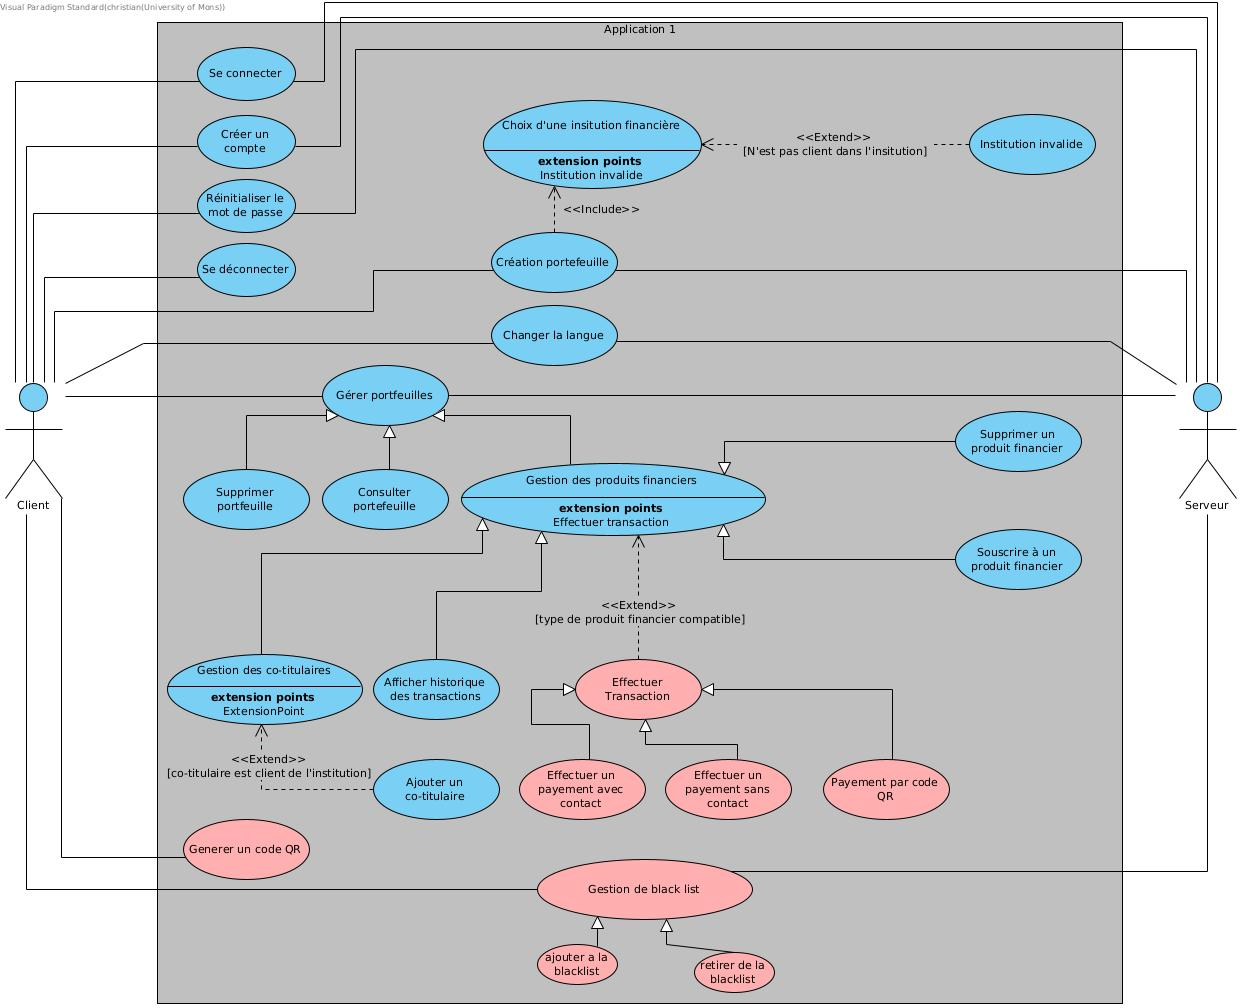
\includegraphics[scale=0.27]{ressources/photos_diagrammes/extensionChristian/usecaseapp1/usecaseapp1.jpg}
						\caption{Diagramme des cas d'utilisation de l'app 1 avec extension}
				\end{figure}
		Pour ce diagramme, j'ai rajouté toutes les nouvelles actions qu'un client pouvais éffectuer.\\
        "Effectuer Transaction" qui comprends "Effectuer un payment avec contact " , "Effectuer un payment sans contact"\\
        et "Payment par code QR" les 3 etant des specialized usecase de "Effectuer une transaction".\\
        J'ai aussi ajouté " Generer un code QR"  et enfin la généralisation " Gestion de black list" avec les specialisations\\
        "ajouter a la blacklist" et " retirer de la blacklist " qui représentent le fait que l'utilisateur peux maintenant définir\\
        et modifier une list de compte à bloquer.
\newpage
		\subsubsection{Interaction Overview Diagram}
			
	    Ce diagramme se base sur celui de l'application 1.

\newpage
		\subsubsection{Diagrammes de classe}
				\begin{figure}[h]
						\centering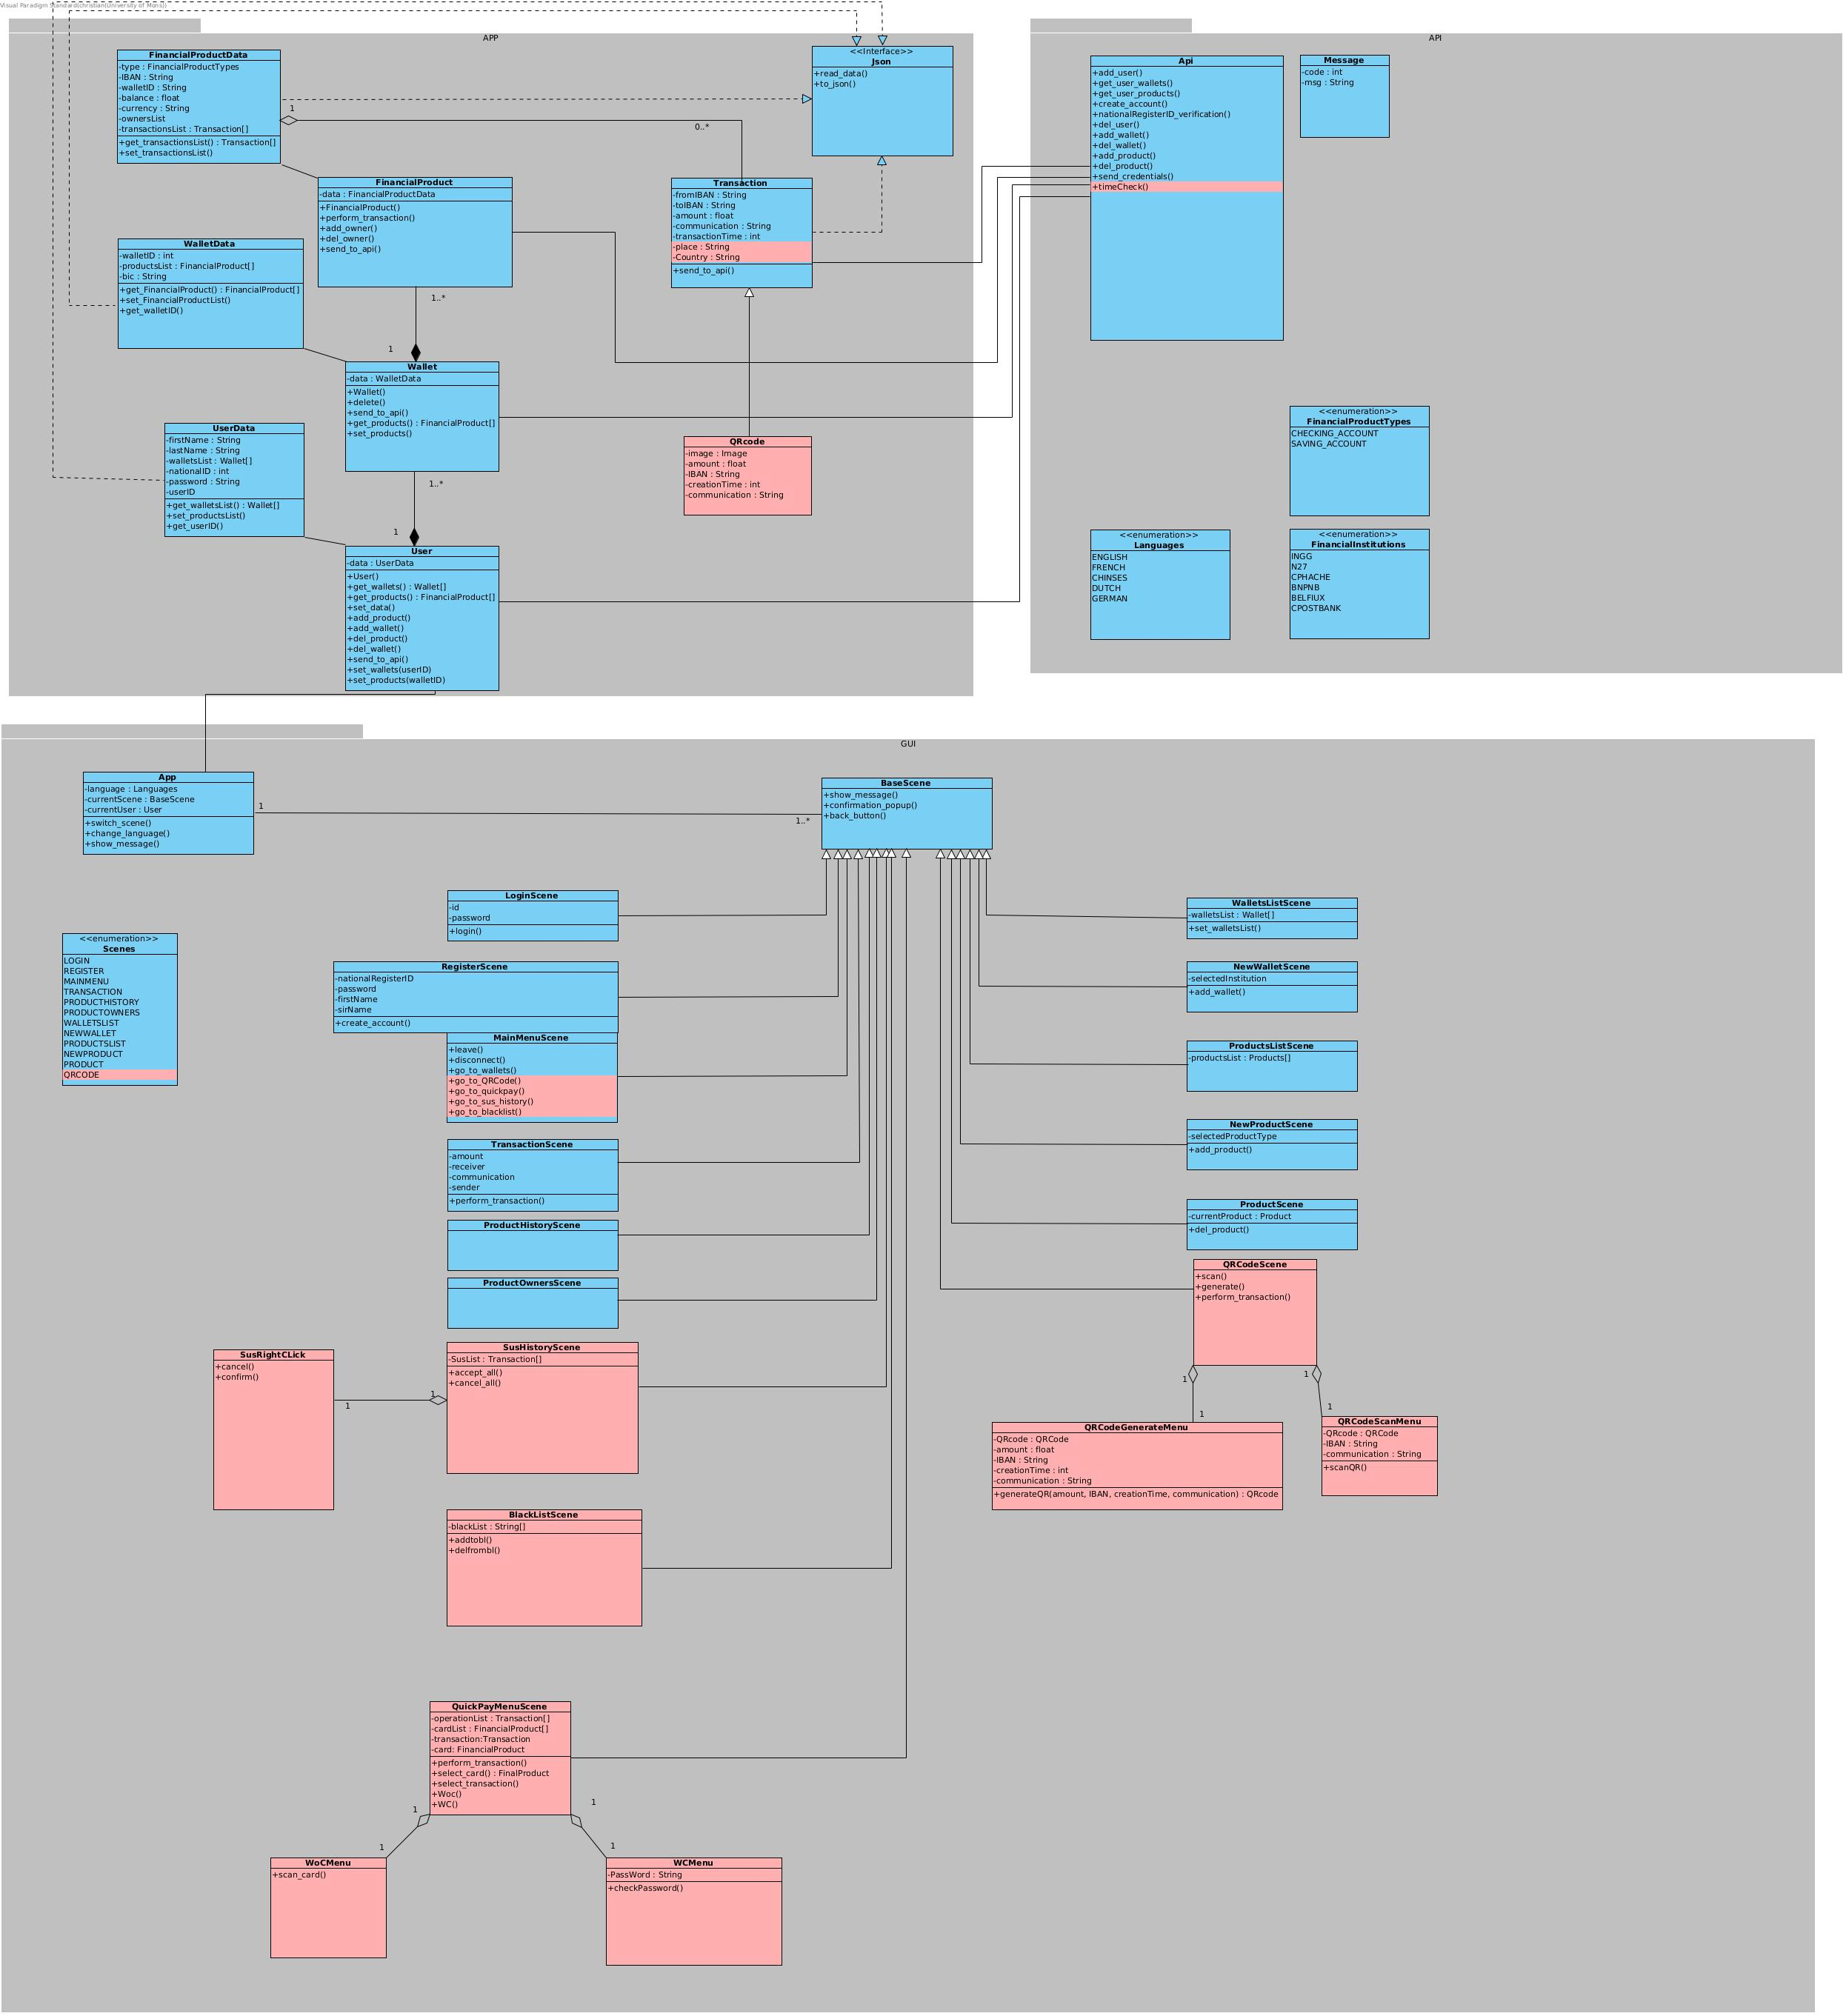
\includegraphics[scale=0.15]{ressources/photos_diagrammes/extensionChristian/classapp1/classapp1.jpg}
						\caption{Diagramme de classes de l'app 1 avec extension}
				\end{figure}
		Dans le package APP de l'application il ne figure q'une seule nouvelle class :\textbf{QRcode}.
        Elle contients les attributs suivant: 
		\textit{image} qui est une objet de type \textit{Image} qui est l'image du code QR. 
        \textit{amount} qui est une objet de type \textit{float} qui est le montant de la transaction.
        \textit{IBAN} qui est une objet de type \textit{String} qui est le compte du receveur.
        \textit{creationTime} qui est une objet de type \textit{int} qui est l'heur et la date de création du QRcode en UNIXTime.
        \textit{communication} qui est une objet de type \textit{String} qui est une communication ( optionel) de la transaction.
		contient également les méthodes liées aux assurances. La classe \textbf{Insurance} est
		\textit{Transaction} qse vois ajouté 2 nouveaux attributs: 
        \textit{place} qui est un objet de type \textit{String} qui est l'endroit du payment, et 
        \textit{country} qui est de type \textit{String} et qui est le pays de destination du virement.
        \bigskip
        Dans le package API je n'ai rajouté que \textit{timecheck} qui est une méthode permetant de verifier le l'heure et la date
        de création d'un QRcode.    

		\bigskip
        Dans le package GUI j'ai rajouté les nouvelles scènes d'ont l'utilisateur a besoin pour :
        Générer un QRcode, scanner un QRcode, effectuer un payment sans/avec contact,gérer sa blacklist.
		
		\subsubsection{Diagrammes de séquence}
				\paragraph{Effectuer une payment avec contact:}
						\begin{figure}[h!]
								\centering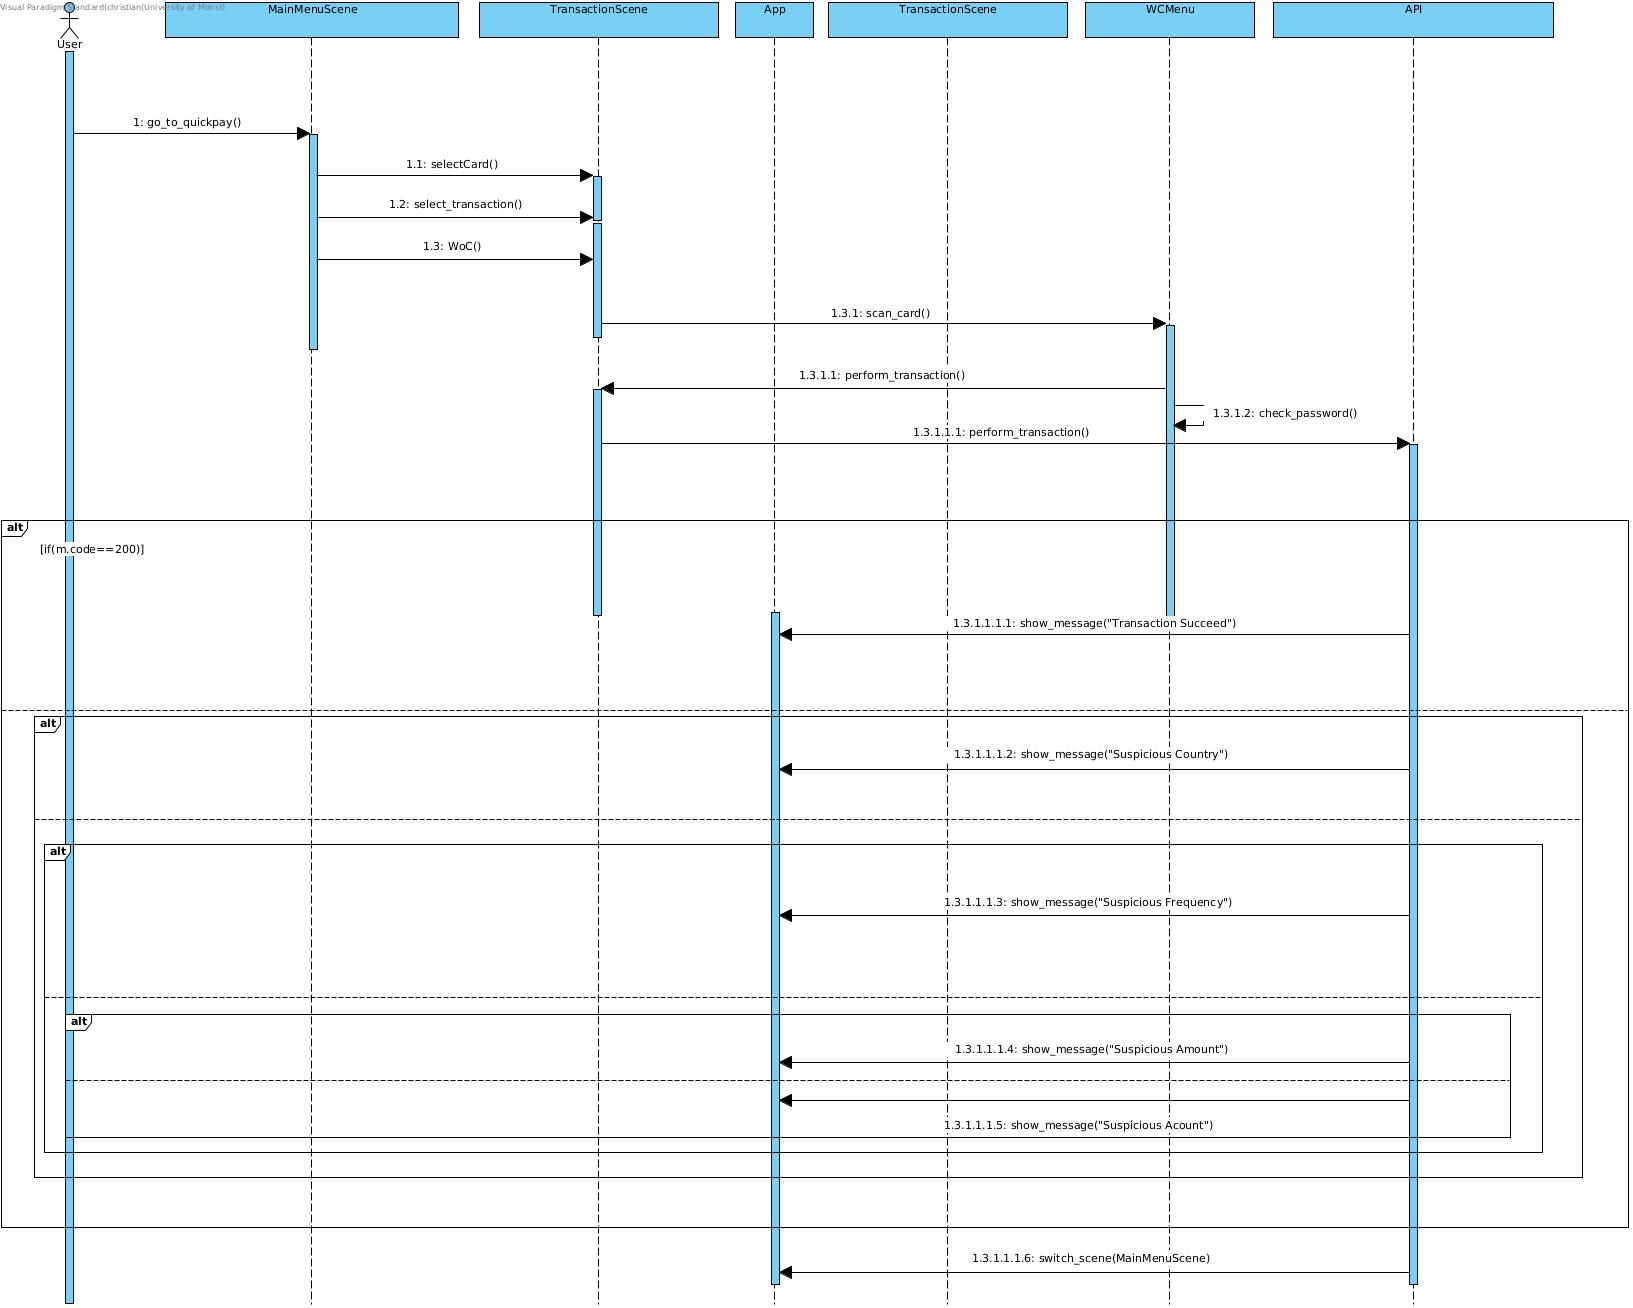
\includegraphics[scale=0.3]{ressources/photos_diagrammes/extensionChristian/interactionapp1/Effecteur_un_payement_avec_contact.jpg}
								\caption{ Effectuer un payment avec contact}
						\end{figure}
					Lorsque le client veux effectuer une payment sans contact il doit tout d'abord selectioner le payment ensuite il choisit
                    le mode de payement avec contact. Après avoir entré le bon code PIN , la  requete de la transaction est envoyé à l'API qui va vérifier la validiter.
                    Si la transaction est suspecte alors elle est soite annulé ou mise en attente de confirmation en fonction du niveau de suspicion.
					\medskip
					Si la transaction n'a pas été effectué le client est notifié avec un message.
                    La procédure est identique pour le payment sans contact hormis le fait qu'en cas de faible suspicion , le mot de passe de l'utilisateur est demandé.
\newpage
			\paragraph{Generer un QRcode}:}
						\begin{figure}[h!]
								\centering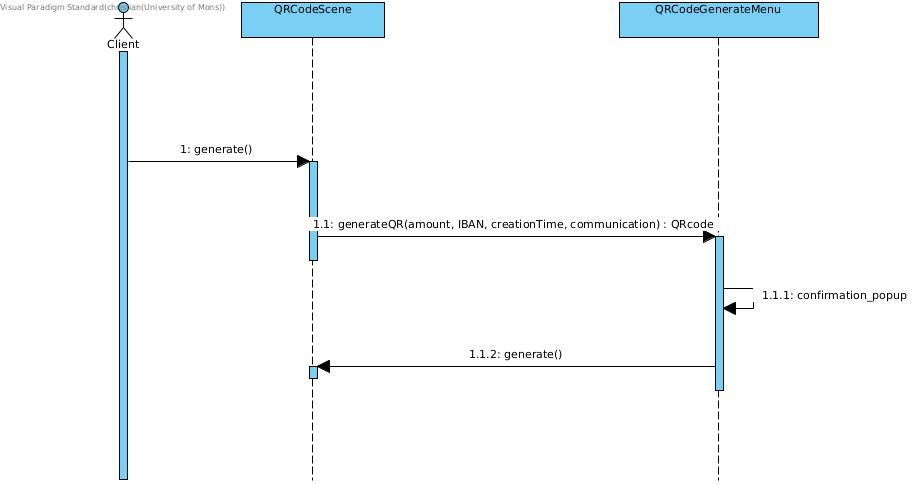
\includegraphics[scale=0.3]{ressources/photos_diagrammes/extensionChristian/interactionapp1/Generer_un_code_QR.jpg.}
								\caption{ Geénère un QRcode}
						\end{figure}
					Le client peut générer un QRcode et elle se stocke localement. Il a pour ça beosin de rentrer le compte sur le quel il souhaite recevoir l'argent,
                    le montant et une communication eventuelle.
					\medskip
					Scanner un QRcode consiste a chager un QRcode et d'éffectuer une transactions a partir de ses informations.	
\newpage		
		\subsubsection{Application 2}
        
		\subsubsection{Interaction Overview Diagram}
        \begin{figure}[h!]

                \centering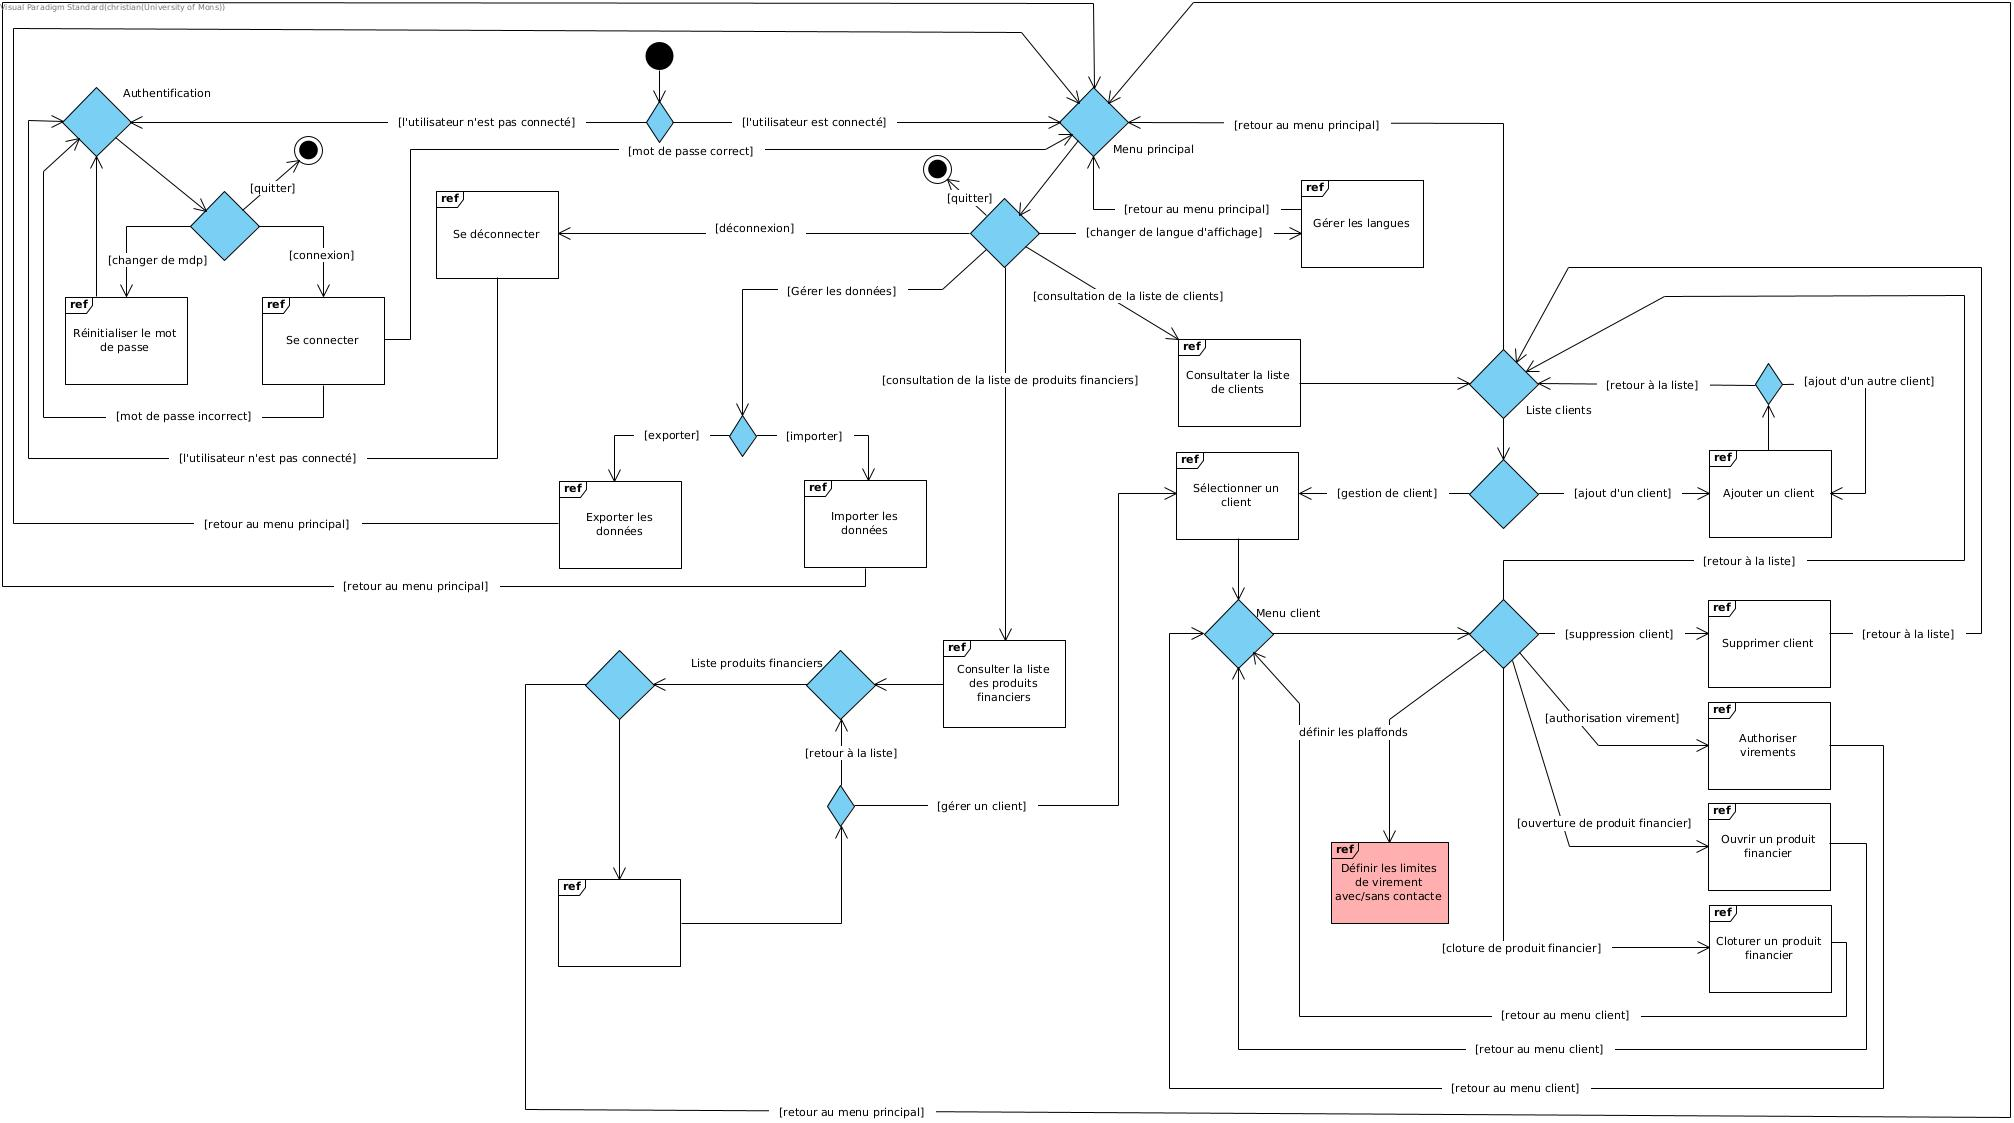
\includegraphics[scale=0.3]{ressources/photos_diagrammes/extensionChristian/interactionapp2/InteractionOverviewDiagram.jpg}
		        \caption{ Interaction Overview App2}
        \end{figure}

        Il n'y a q'un seul cas rajouté a ce diagramme. Ce cas réfère a la gestion de limites sur les payments avec et sans contact.

		\subsubsection{Diagramme de classes}

				\begin{figure}[h]
						\centering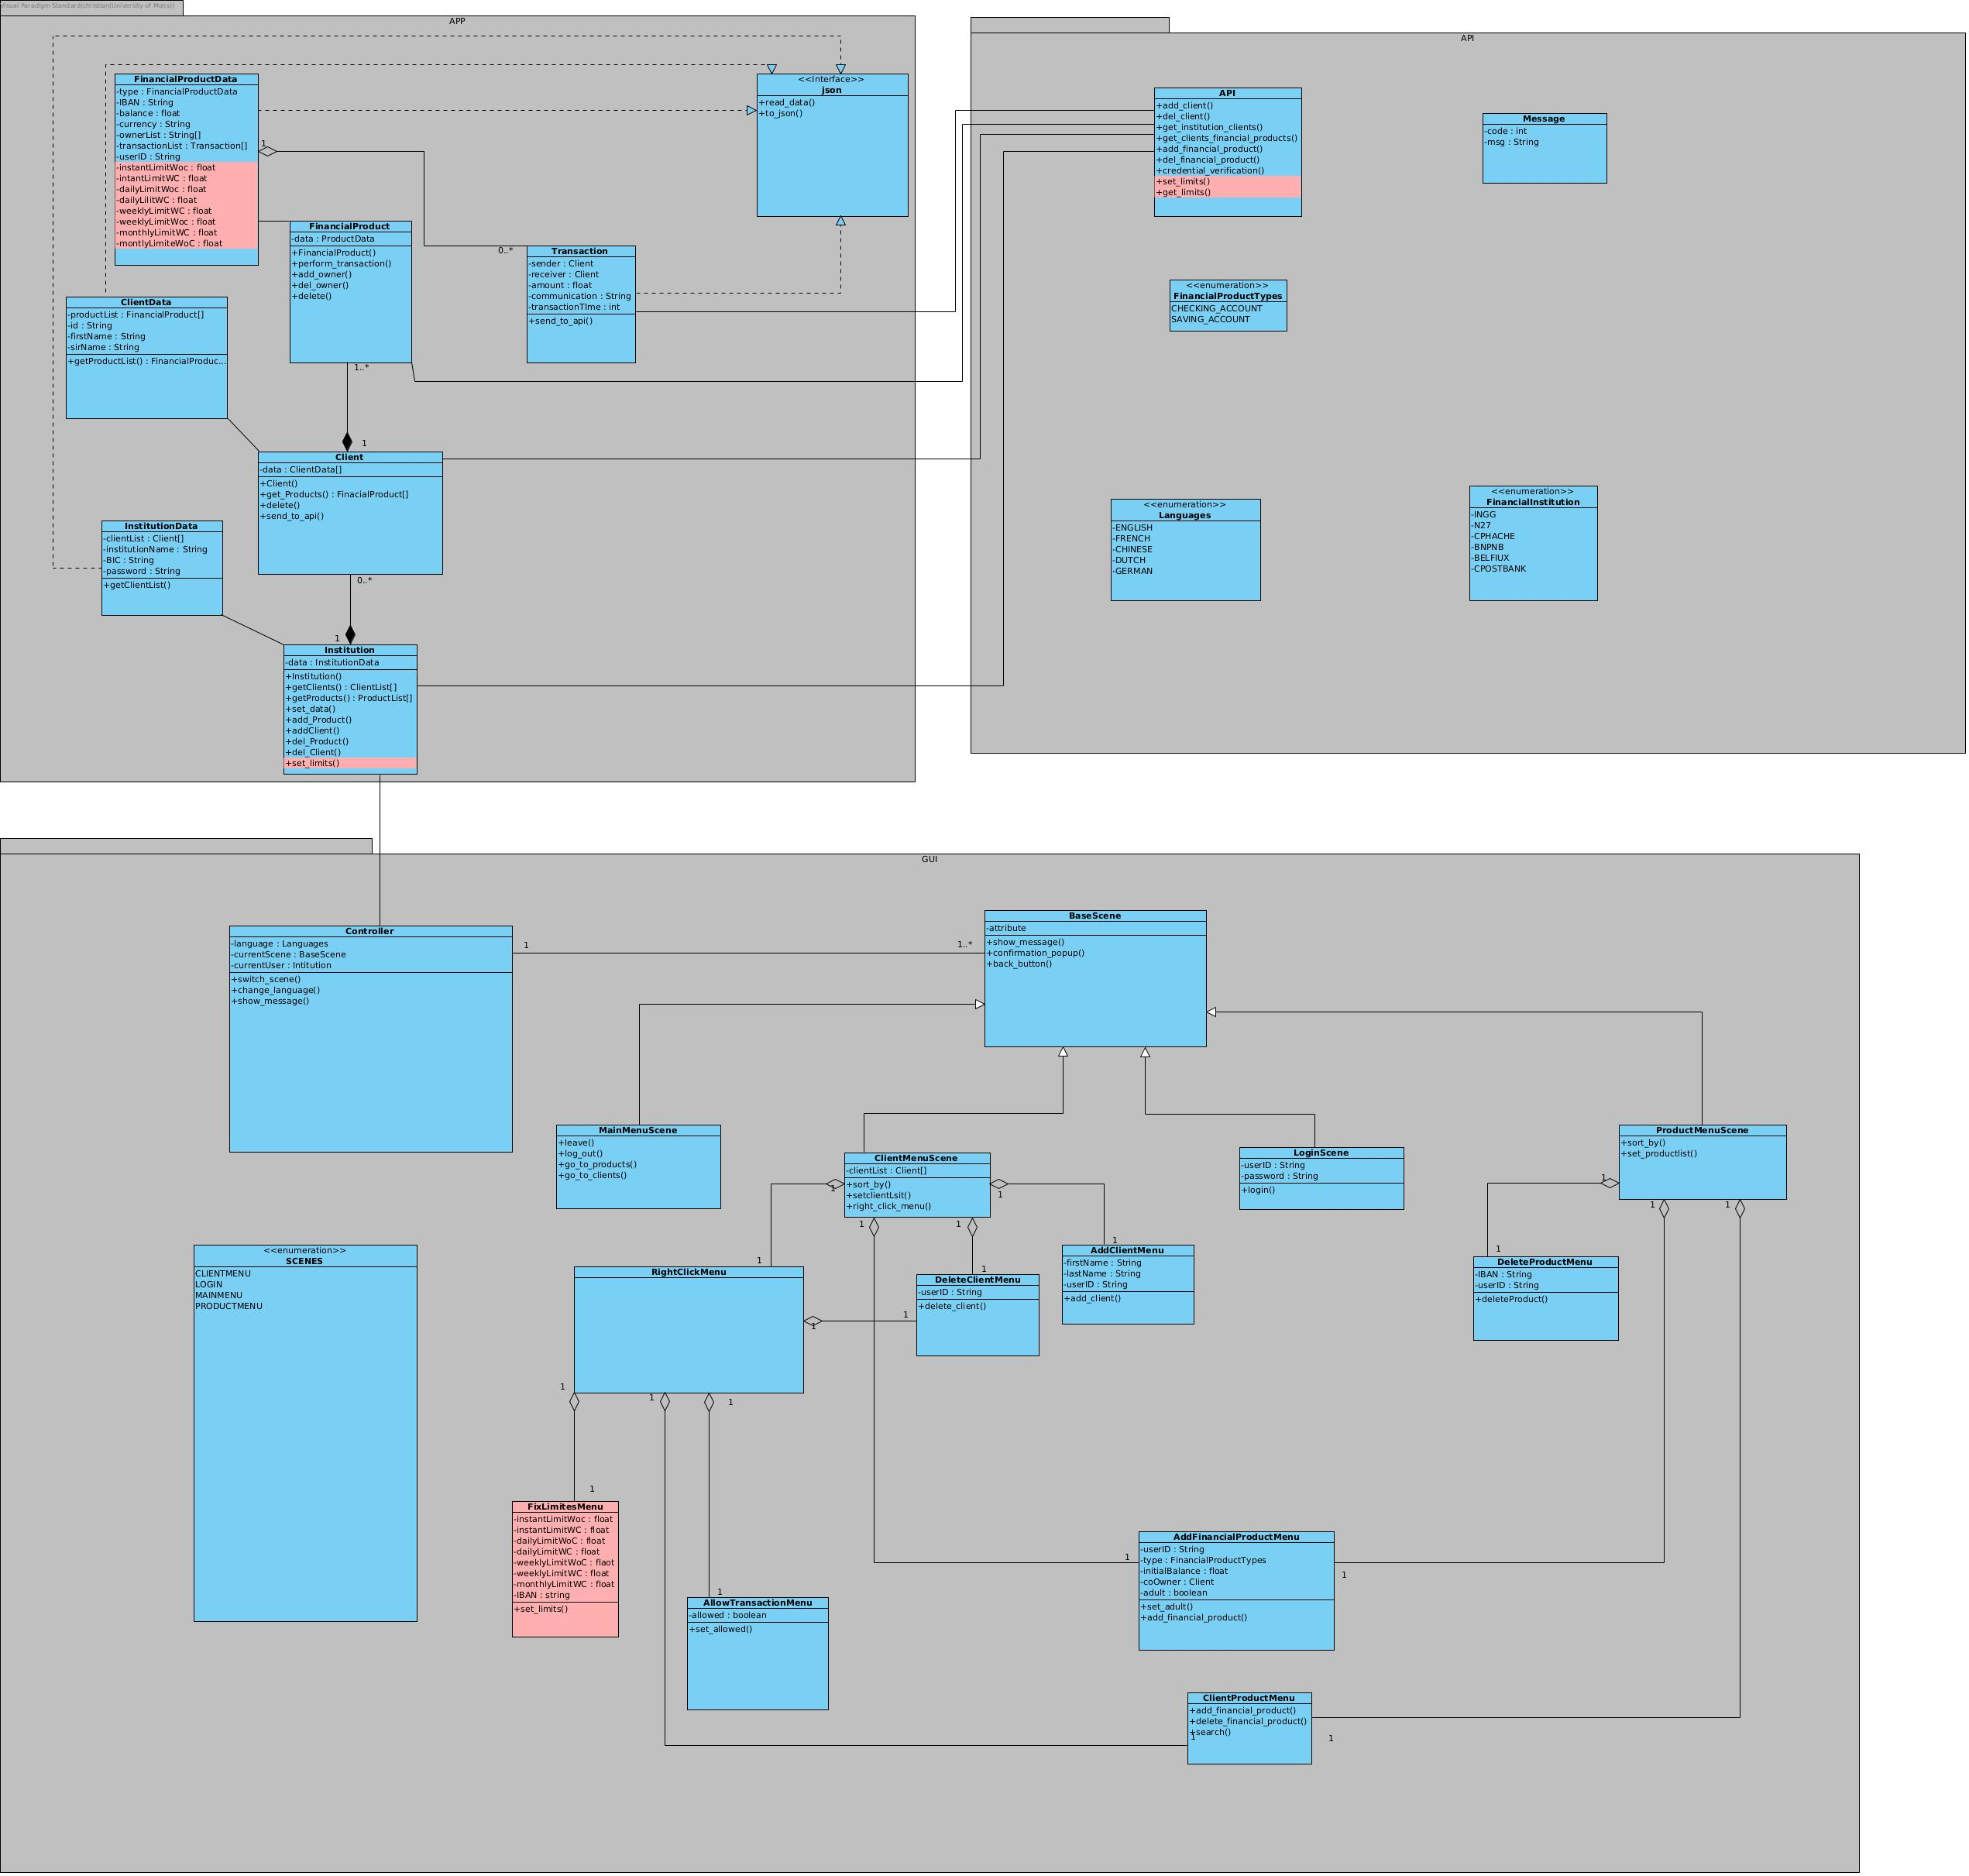
\includegraphics[scale=0.15]{ressources/photos_diagrammes/extensionChristian/classapp2/ClassDiagram.jpg}
				\end{figure}
		Dans le package App j'ai rajouté des attributs référant au diffèrent types de limites qui peuvent être mise sur les virement avec ou sans contact.
        L'objet \textit{Institution} possède désormais une méthode permettant de définir les limites des virment avec ou sans contact nomée \textit{set_limits}.

		\bigskip

		L'API contiens maintenant des méthodes permetant d'envoyer \textit{set_limts} et de recevoir \textit{get_limits}
        du serveur.

		\bigskip

        Dans le package GUI j'ai rajouté la scène permettant aux employés des instituions de définir les plafonds de transactions.
		\medskip

\newpage
		\subsubsection{Diagrammes de séquences}
				\begin{figure}[h]
						\centering\includegraphics[scale=0.3]{ressources/photos_diagrammes/extensionChristian/interactionapp2/Définir_les _limites_de_virement_avec_sans_contacte.jpg}
						\caption{Définir les plafonds sur les virement avec ou sans contact}
				\end{figure}

				Si l'employé d'une institution a besoin de définir des plafonds sur les virement avec ou sans contact il peux le faire en effectuant un clique droit sur le menu des clients.
                Grace à ça il a maintenant accès à différentes options parmis lesquelles se trouve la définitions de limits. En cliquant dessus , il poura entrer les différentes valeurs
                des limites souhaitées et confirmer celles-ci. Après confirmation, la GUI au travers de la méthode \textit{et_limits()} d'Institution va envoyer ces limites à l'API.
                
\newpage
		\subsubsection{Serveur}
		\subsubsection{Diagramme d'entité relation}

				\begin{figure}[h]
						\centering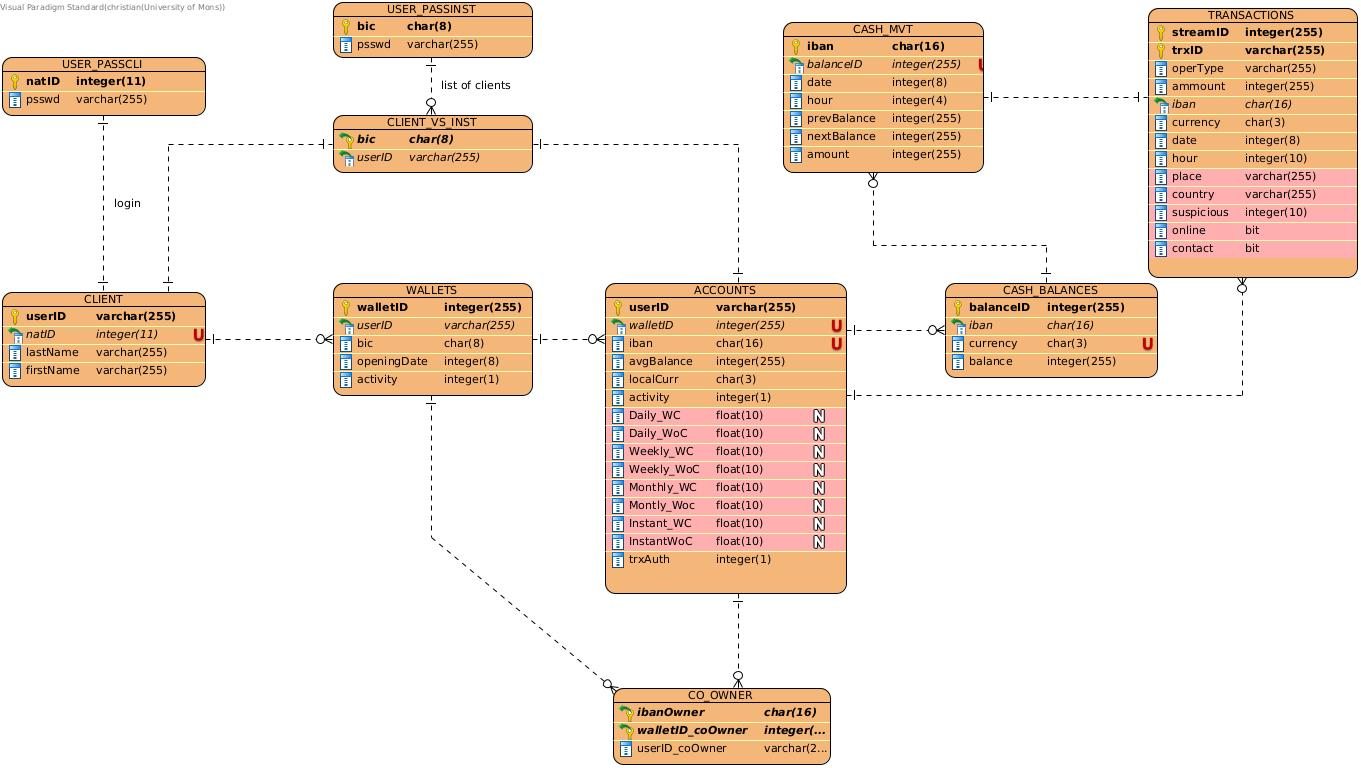
\includegraphics[scale=0.25]{ressources/photos_diagrammes/extensionChristian/erd/EntityRelationshipDiagram1.jpg}
						\caption{Diagramme d'entité relation avec extension}
				\end{figure}
		Le diagramme d'entité relation a été étendu à l'aide de 8 attribut dans la table \textit{ACCOUNT} et de 5 attributs dans la table \textit{TRANSACTION}
				
		\medskip

		Les nouveaux attributs de la table \textit{ACCOUNT} sont les limites qui peuvent être définis ppur les virement avec ou sans contact 
        Les nouveaux attributs de la table \textit{TRANSACTION} servent a la detection de fraude.

		
\end{document}
